\documentclass{article}
\usepackage{geometry}
 \geometry{
 a4paper,
 total={140mm,247mm},
 left=35mm,
 top=25mm,
 }
 \usepackage{todonotes}
\usepackage{graphicx}
\usepackage{caption}
\usepackage{subcaption}
\usepackage[]{threeparttable}
\usepackage{url}
\begin{document}
\title{Assessing decentralization is DPoS environments\\ \small{Draft}}
\author{\normalsize Tarek Awwad, Julien Guyomard, Reda Berrehili\\Ki Foundation\\\small\{\textit{[first]}@foundation.ki\}}
\maketitle

\begin{abstract}
\end{abstract}
Decentralizing the validation process in blockchain environments is a pillar of the fairness, security and liveness promises of this technology. Although, the literature provides neither a clear formal definition of decentralization nor a practical tool to measure it. In this document, we identify and define the facets of the decentralization in blockchain systems and leverage a couple of techniques that allow to assess its extent in DPoS systems.

\section{Introduction}
\label{sec:intro}
The Delegated Proof of Stake consensus protocol (DPoS) consists in transferring the validation power - expressed in terms of monetary stake - from the node community to a reduced committee of trusted nodes selected through a voting process. This system has proven its efficiency from the energetic and performance perspectives when compared to the Proof of Work and Proof of stake based consensus algorithms respectively. Moreover, theoretically speaking, the technical foundations and specifications of the DPoS algorithm (in its different variants), strive at guaranteeing a resilient validation process to improve the security and liveness of the blockchain. Nevertheless, the practical experience has shown that this goal might not be straightforwardly achievable due to various reasons.

\subsection{Limitations of DPoS}
In fact, it is fairly easy to identify the potential vulnerabilities and weaknesses of DPoS by comparing its functioning to more similar traditional and well established decision making systems such as political and administrative ones. For instance, in parliamentary systems, a badly conceived or corrupted voting law can yield (i) a non-representative vote-whales-driven parliament in which, decisions are made based on the interest of those vote whales, (ii) a corrupted parliament where deputies legislate to their own benefits or (iii) a "perpetual" parliament whose members legislate to maintain the power by leveraging their positions to be re-elected. All this translates, in DPoS, as follows:

\paragraph{Whales} Wallets or wallet coalitions which possess a large proportion of the token staked in the system, can unilaterally decide the fate of one or multiple validators which gives them the ability to introduce corrupted validators or to establish an accountability system allowing them to influence the behaviour of their delegated validator or to bias the votes of other smaller wallets.

\paragraph{Stationary votes}
The current implementations of the voting/staking procedures in the existing DPoS blockchains aim at providing the user with an easy and straightforward way of voting and unvoting validators. However, observing the voting behavior of the wallets shows that a small minority of them actually keeps track of the performance and reliability of the validators and adjusts their vote accordingly. This can be noticed in the ARK blockchain\footnote{\url{https://ark.io}}, for example, where some validators stays offline for a couple of days without actually loosing a consistent number of votes \footnote{In the ARK blockchain, where 51 validators constitutes the validation committee, a validator stays in the top 51, regardless their actual availability, as long as they accumulate enough votes to be in the top-51.}. This lack of reactivity form the voters renders the voting system useless and thus, helps promoting new security vulnerabilities in the blockchain (as it then tends to a Proof of Stake system with a very limited number of validators).

\paragraph{Equilibrium} Naturally, a direct result of a voting based system is the emergence of a competition between validation candidates who seek to attract the wallet votes by incentivizing them through higher payout or deeper contribution in the code reviewing and improvement. While the latter concerns a small part of the community (a.k.a. enthusiasts), the former concerns a wider group of wallet holders and constitutes the real differentiation criterion between the candidate proposals. However, in practice, as the range in which this payout can change is narrow, this impact of this competition is limited and the reasons for a wallets to change its vote are restricted. This added to both the stationary votes and the unbalanced whale weight would eventually lead the system to reach a Nash equilibrium \cite{maskin1999nash} in which no actor has the benefit to unilaterally change its behavior (e.g. using the same payout True Block Weight algorithm by all the delegate in the ARK blockchain).

The aforementioned elements describe in reality the convergence of the system toward a centralized and constrained validation committee. This renders it, in practice, closer to a centralized server-based system with high redundancy. Accordingly, in this case, the blockchain might inherit the vulnerabilities of a centralized architecture such as a higher corruption risk and a higher potential for attack (since the validators are exposed and not changing).

\subsection{The decentralization facets}
In order to be able to assess the decentralization in a blockchain, one needs first to identify the domain specific facets of this decentralization.

\paragraph{Number of validators per round}
This is the number of validators that should agree on transactions and blocks in each round. Indeed, the higher this number is, the lower the risk of compromising the integrity of the blockchain by compromising a subset of these validators is. This has been commonly considered the main factor reflecting the decentralization in a DPoS system.  However, while important, the number of validators per round is not satisfactory by itself. To illustrate this, one can compare 2 blockchains with a low number of validators per round with the difference that for the first these validators are unchanged between rounds and for the second these validators are constantly changing between rounds. It is clear that these 2 blockchains have two different degrees of decentralization and of risk factors.

\paragraph{The size of the validator pool}
The validator pool refers to the set of all nodes that could be selected as member of the validator list. They are nodes that fulfilled the candidature requirements (e.g., the delegate registration in ARK). Mathematically speaking, regardless of the used selection method, a smaller pool will yield more similar validator lists between validation cycles/rounds than a larger pool. Which in truns, means that the validation power will be more concentrated. Moreover, A pool of a smaller size limits the choice of the wallet during the voting and thus decreases the amount of accountability that the voting system is meant to provide.

\paragraph{Collusion factor} This defines to what extent validators are potentially forming coalition to bias the block validation process and thus compromising the integrity and security of the blockchain. Indeed, a lower number of validators per round increases the probability and impact of the existence of such a coalition. However, other design elements are also important such as the resiliency to Sybil attacks, the reliability-independent randomness in the validator selection, etc...

%\paragraph{The predictability factor} This defines how predictable is the next validating pool is. A highly predictability can allow attackers to

\paragraph{Stability duration} This defines the time during which the set of validator is unchanged. A longer stability period indicates a more centralized system. This range in which the value of this factor is considered acceptable is not absolute and depends on the configuration and the functioning rule of each blockchain. One can use relative time unit such as rounds to have a better means of comparing different blockchains. However, this is not satisfactory to englobe more complex system architecture based on cycles, sharding and so on.

\section{Related work}
In this section, we give a fast overview of existing works aiming at defining and assessing the decentralization. In PoW systems, the decentralization is commonly linked to the hashing power of the miners. Miller et al. studied in \cite{miller2015discovering}, the presence of influential nodes in Bitcoin and found that a small fraction of the network, containing around 100 nodes,represents more than 75\% of the mining power.In \cite{gencer2018decentralization}, the authors compares the decentralization in Bitcoin and Ethereum. To this end, this work provides a study on the network level aspects of the mining process such as bandwidth, latency, P2P latency, etc. as well as on the hashing power and the number of pruned blocks.   In \cite{gervais2014bitcoin}, Geravis et al. consider a larger scope for decentralization in Bitcoin which not only covers the mining power but also show that a limited set of entities control also the services, decision making and the incident resolution  processes. In DPoS, existing methods mainly focuses on the number of validators per round and the size of the validator pool. In \cite{kwon2019impossibility}, authors extensively studies DPoS systems from a diversity and wealth distribution perspective using tools such as the \textit{Gini} index . Finally, in \cite{DecentralizationCrypto}, the author leverages the Herfindahl–Hirschman Index\cite{rhoades1993herfindahl} to measure the decentralization. However, this study tackle the decentralization as a measure of project diversity in the crypto-space and not the diversity of validator/block-producer within a blockchain.

\section{Experimental setup}
In the remainder of this document, a set of techniques that allow measuring the decentralization of DPoS systems is proposed. In order to show how these techniques behave on real world data, we consider hereafter the validation data of two common blockchains: the ARK blockchain and the LISK\footnote{\url{https://lisk.io/}} blockchain. In ARK each validation round englobes 51 validators. We considered the blocks validated since the launch of the system until June 2019 which is equivalent to 8.7 million blocks and 170K validation rounds. On the other side, LISK uses 101 validators per round and the data considered covers the whole life time of the blockchain untill july 2019. That is, 9.8M blocks validated during 96K rounds. For convenience, the experiments shown below where performed on a sample of the data described above. The sampling process consists in randomly picking one validation round per week (resp. day) which reduces the number of considered observations (i.e. rounds) to arround 120 rounds (resp. 810 rounds) for ARK and 150 (resp. 1100 rounds) for LISK. After the sampling, we ended up with 170 unique validators for ARK and 266 unique validators for LISK \footnote{These are validators who validated at least one block. Registered validators who never validated any block are not considered.}. Table \ref{tab:data} summarizes the characteristics of the used datasets.

\begin{table}[]
\centering
 \begin{threeparttable}
 \begin{tabular}{|c c c c c|}
 \hline
 Blockchain & \#Val. (U) & \#Val. (R) & \#Rounds & \#Blocks  \\ [0.5ex]
 \hline\hline
 ARK & 171 & 51 & 170K & 8.7M  \\ [1ex]
 ARK (Days)  & 162 & 51 & 810 & - \\ [1ex]
 ARK (weeks) & 132 & 51 & 120 & - \\ [1ex]
 LISK & 280 & 101 & 96K & - \\[1ex]
 Lisk (Days) & 270 & 101 & 1100 & - \\ [1ex]
 Lisk (weeks) & 266 & 101 &150 & - \\ [1ex]
 \hline
 \end{tabular}
     \begin{tablenotes}
     \centering
      \small
      \item Val. (U): Unique validators, Val. (R): validators per Round
      \item Data collected form 04.17 to 06.19 (ARK) and from 05.16 to 07.19 (LISK)
    \end{tablenotes}
 \end{threeparttable}
 \caption{An overview of the datasets used in the experiments}
 \label{tab:data}
\end{table}

To these real datasets, we added a synthetic dataset simulating a random selection. From the same list of unique validators as ARK, we generated new validation rounds by randomly selecting 51 validators at each round. We then doubled the size of the candidate pool (unique validators) by appending newly created unqiue validators and generated another random configuration using the same procedure as before. This yielded two new datasets summarized in Table \ref{tab:dataR}.

\begin{table}[]
\centering
 \begin{tabular}{|c c c c|}
 \hline
 Configuration & \#Val. (U) & \#Val. (R) & \#Rounds   \\ [0.5ex]
 \hline\hline
 Random & 162 & 51 & 810 \\ [1ex]
 Random (High) & 324 & 51 & 810  \\ [1ex]
 \hline
 \end{tabular}

 \caption{An overview of the Random synthetic datasets used in the experiments}
 \label{tab:dataR}
\end{table}

\section{Inter-round agreement}
\label{sec:agreement}
We are interested in capturing the stability in the validator list over time. That is, how many common validators one can find between rounds. In other words, how much the rounds agrees between each others on who should be part of them and who should not. In fact, one can do the analogy with systems where the agreement of a set of users over a set of units needs to be computed e.g. rating systems, fact checking systems, descriptive vote analysis, etc. In the case of the validation process, users are the rounds and the units are the validator. That is each round $i$ answers the following question: should a validator $j$ take part of the round $i$ itself? Using the historical validation data, one can build a decision matrix $D$ where rows are rounds and columns are unique validators and where a coefficient $D_{ij} = 1$ if validator $j$ participated in round $i$ and $D_{ij} =0$ otherwise.

Second, an agreement measure can be used to measure how similar the rounds are. Here we choose to use the Krippendorff's alpha \cite{krippendorff2018content} which is an agreement measure that normalizes the observed disagreement with the expected disagreement (based on a random distribution of the observed answers). This measure has been described by Belfodil et al. \cite{belfodil2019dEV} as follows (where $\alpha$ denotes the krippendorff's alpha):


\textit{The core idea is that a proper measure would be: on a scale from the
contingency table of chance agreement to the contingency table of maximum agreement, how
far along that line do we find the contingency table of observed agreement? More formally:
\begin{center}
$observed co-occurrences = \alpha(maximum agreement)+(1 - \alpha)(chance agreement)$
\end{center}
Hence, when $\alpha$ = 1, the agreement is as large as it can possibly be (given the class prior),
and when $\alpha$ = 0, the agreement is indistinguishable to agreement by chance.}\\

We computed the krippoendorff's alpha for the ARK and LISK blockchains. For reference we also used the random configuration described earlier. Naturally for the random validator selection is supposed to yield a low agreement between the rounds. It is computed alpha was indeed equal to 0. On the other hand, the agreement for LISK ($\alpha_{LISK}$) was equal to 0.45 and the agreement for ARK's rounds ($\alpha_{ARK}$) was equal to 0.46. Which is comparably similar. This shows that the agreement between the different rounds is fairly high which indicates a possible partial centralization of the validation process. It is clear that, while this compact measure gives a clear indices on a relative centralization, is not sufficient to capture a more detailed view on the facets that induces this centralization. Ways of improving this appraoch are discussed latter in this document.

\section{Density based clustering}
\label{sec:dbc}
An other way of assessing the similarity between the rounds (as validator vectos) is clustering. Clustering consists in grouping the elements of a set, each described by a vector of attributes, into homogeneous categories w.r.t. to a predefined distance measure and cost function. There are essentially 3 families of clustering algorithm\footnote{We consider only the deterministic clustering approaches.}: partitioning clustering, hierarchical clustering and density based clustering. They can be summarized as follows:

\paragraph{Partitioning clustering} As defined in \cite{Jin2010} a partitional clustering decomposes a data set into a set of disjoint clusters. Given a data set of $N$ points, a partitioning method constructs $K$ ($N \geq K$) partitions of the data, with each partition representing a cluster. That is, it classifies the data into $K$ groups by satisfying the following requirements: (1) each group contains at least one point, and (2) each point belongs to exactly one group. A well known clustering algorithm belonging to this category is K-means.

\paragraph{Hierarchical clustering} \cite{murtagh2014ward} In the agglomerative version of this approach, each data point is, initially, considered as an individual cluster. At each iteration, close clusters are merged together until one cluster or $K$ clusters are formed. This allows to build a cluster tree for different values of $K$. On the other hand, the divisive hierarchical clustering, all the data points  are considered to belong to one a single cluster and in each iteration, the parent clusters are split into smaller cluster with more similr points.

\paragraph{Density based clustering} Density based clustering such as DBSCAN \cite{ester1996density} requires two parameters: $eps$ which is the maximal distance between 2 vectors to consider them as neighbors and the minimum number of neighbor vectors ($minPts$) required to form a dense region i.e., a cluster. It starts with an arbitrary starting point that has not been seen before by the algorithm. Its $eps$-neighborhood is computed and  a cluster is started if the neighborhood contains at least $minPts$ points. Otherwise, the point is labeled as a local noise (i.e., w.r.t. to the current cluster. It, however might be later assigned to another cluster if it belongs to a sufficient neighborhood.).

Both the partitioning and hierarchical clustering are ruleds (to different extents) by an input number of cluster to produce. When this number of cluster is set to one, all the points are gathered into the same cluster. This is not adapted to our use case as our aim here is to discover a concentration of similar round vectors and not to partition the whole space. That is, if any outliers exist (i.e. vector wich are not similar to any other vectors), we would rather leave them aside as they can be considered as noise. Accordingly, DBSCAN is a perfect candidate to achieve this task. In practice it is fairly difficult to find the right values of the $eps$ and $minPts$ parameters. Therefore, in our case, we study the output of clustering the round vectors for the whole range of possible values for both parameters. In a centralized system, one can expect to find one fairly big cluster (i.e., with low noise) for a low value of $eps$ and a high value of $minPts$. Whereas for a more decentralized system, one can expect to have a high number of outliers and few vectors belonging to the same cluster except for very loose values of $eps$ and $minPts$ (i.e. very high $eps$ and very low $minpts$). Figure \ref{fig:db} depcits the results of clustering the ARK rounds and the LISK rounds while Figure \ref{fig:dbRan} the clustering of the randomized rounds described in Section \ref{sec:agreement}. Values of $eps$ in $[0,1]$ are considered wit steps of $0.05$ and vlaues for $minPts$ between 5 and 200 are considered with steps of 8. For each configuration we report the silhouette measure indicating the quality of the clusters\footnote{Values in $[-1,1]$, where 1 indicates very high quality clusters, 0 indicates random clusters and -1 indicates that the vectors were assigned to bad clusters.}\cite{rousseeuw1987silhouettes}, the number of generated clusters and the number of outliers. Note that the used clustering distance is the Jaccard distance \cite{levandowsky1971distance} and the data used are those relative to the day based sampling to provide enough data points to the clustering algorithm.

To interpret the figures, for each blockchain, one should first look at the silhouette heatmap and identify high quality clustering (darker green). Then, one should consider the number of clusters and noisy points generated within this high quality clustering region. A number of clusters close to 1 and a low number of  outliers indicate a centralized validation process if the considered region (dark green) is determined by a low $eps$ and a high $minPts$. Accordingly, we can observe that the randomized rounds configuration is fully decentralized (no dark green regions) which is expected\footnote{This is an extreme case provided as an example. Indeed, a complete random selection is equivalent to high security risks and must be avoided even if it provides high decentralization.}. While in the cases of ARK and LISK, one can identify more interesting patterns which can be summarized as follows: when clustering ARK rounds, the intersection between the good quality clustering region the low number (up to 2 clusters) of clusters and on noise points (between 0 and 300) is restricted by $eps \in [0.23, 0.35]$ and $minPts \in [93, 133]$. While for LISK, these intervals are wider and most importantly covers lower values of $eps$ and $minPts$ while maintaining a low number of outliers. The comparison of those observations suggests that LISK, despite have a higher number of validator per round, is more centralized than ARK as its validator list changes less frequently from one round to another.

\begin{figure}
     \centering
     \begin{subfigure}[b]{\textwidth}
         \centering
         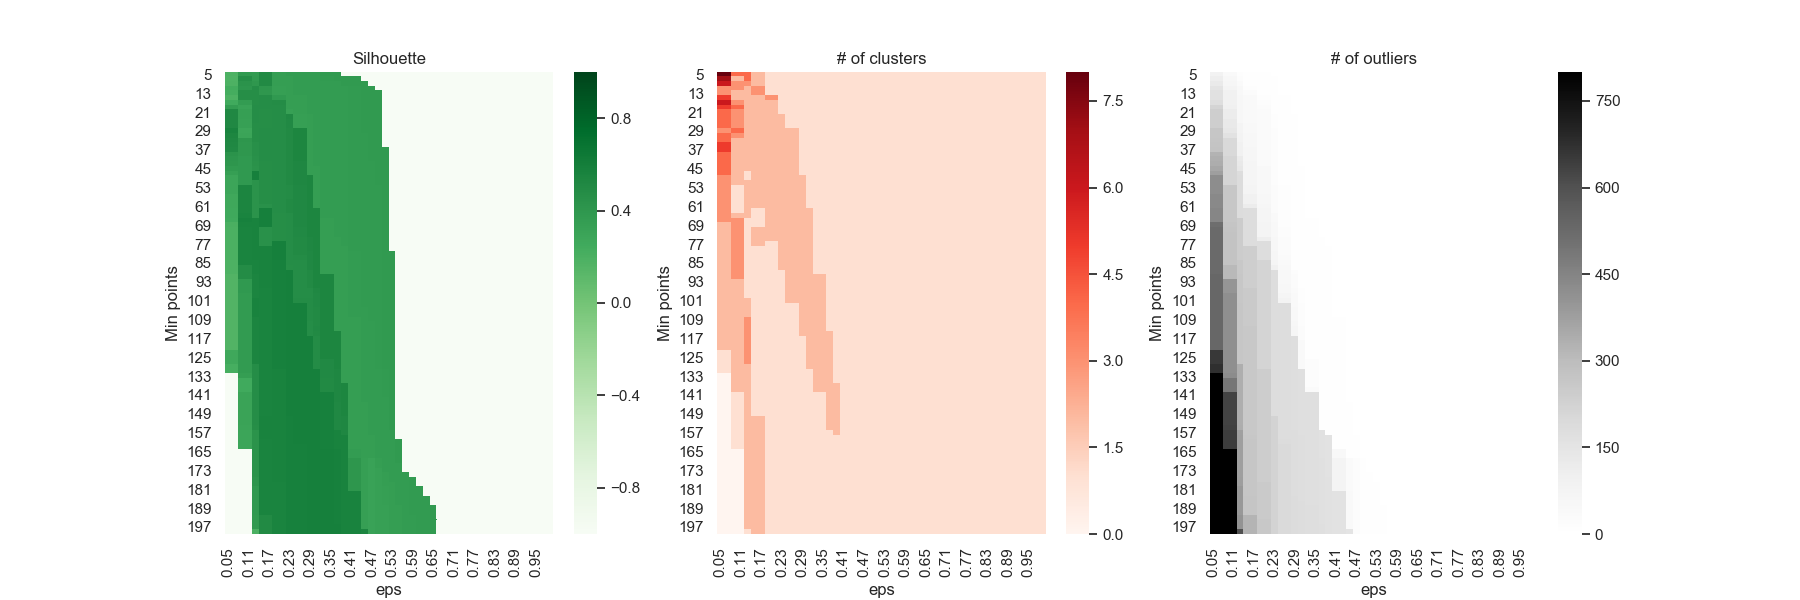
\includegraphics[width=\textwidth]{figures/RealN.png}
         \caption{Validator selection in ARK}
         \label{fig:DBARK}
     \end{subfigure}
     \hfill
     \begin{subfigure}[b]{\textwidth}
         \centering
         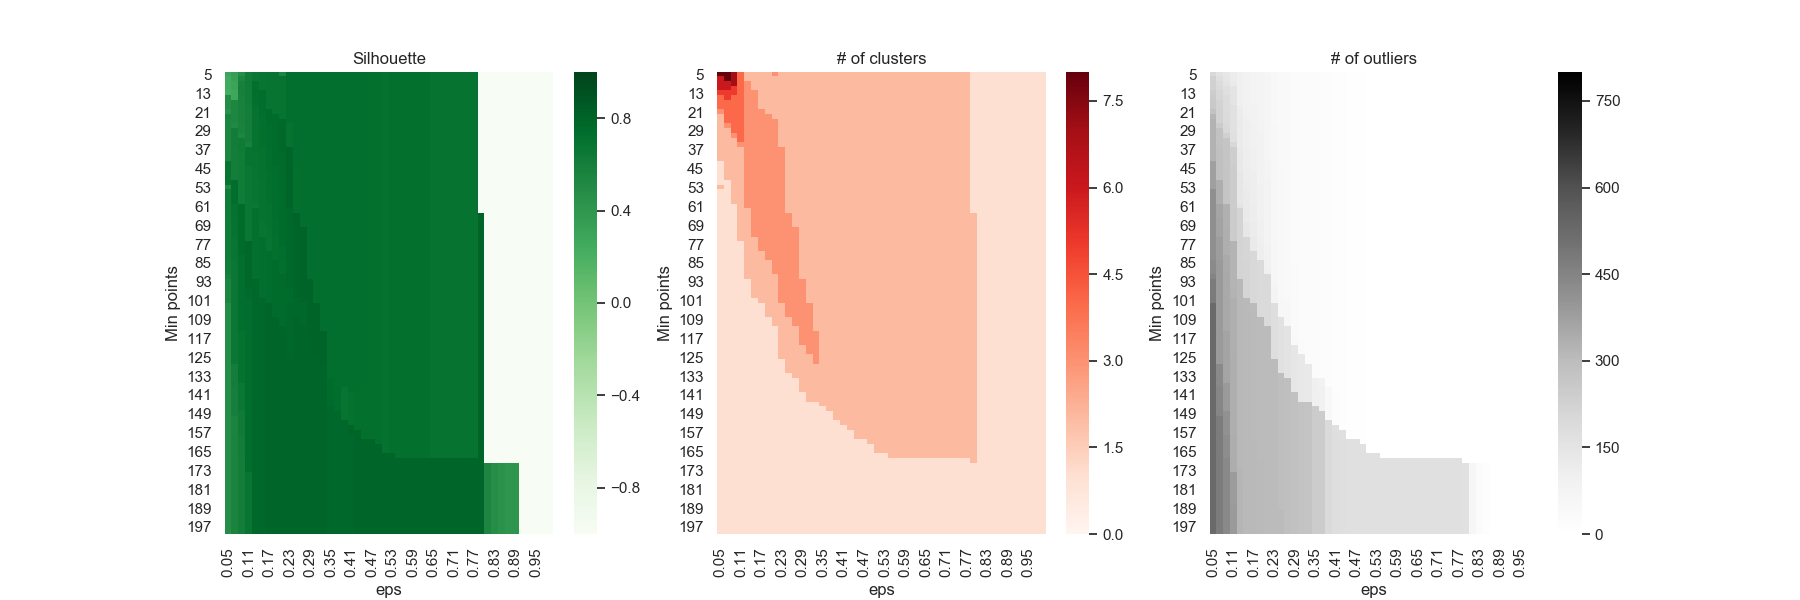
\includegraphics[width=\textwidth]{figures/LISK1dayNameN.png}
         \caption{Validator selection in Lisk}
         \label{fig:DBLISK}
     \end{subfigure}
    \caption{The silhouette, number of clusters and number of outliers for different values of $eps$ and $minPts$ for real data.}
        \label{fig:db}
\end{figure}

\begin{figure}
     \begin{subfigure}[b]{\textwidth}
         \centering
         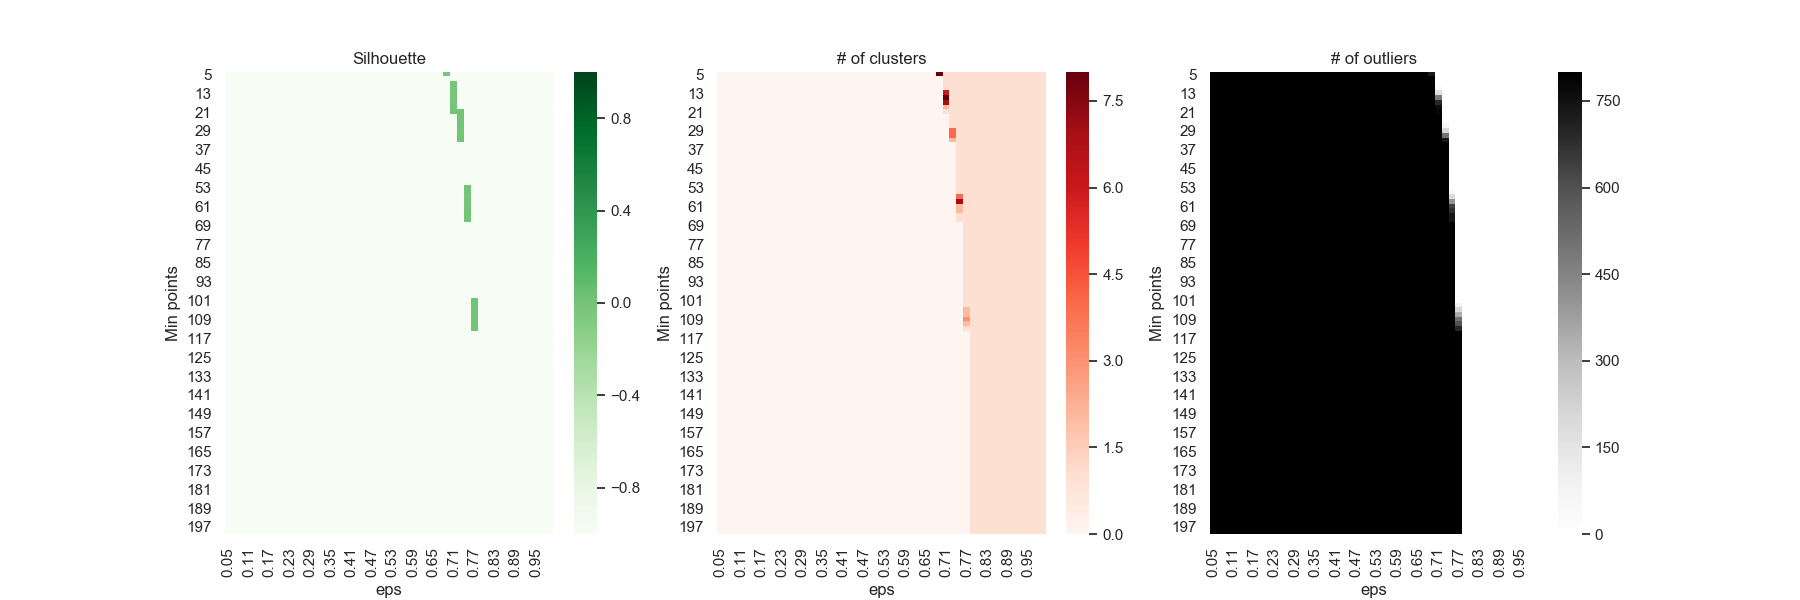
\includegraphics[width=\textwidth]{figures/Rand.png}
         \caption{Random validator selection}
         \label{fig:DBRAN}
     \end{subfigure}
         \hfill
     \begin{subfigure}[b]{\textwidth}
         \centering
         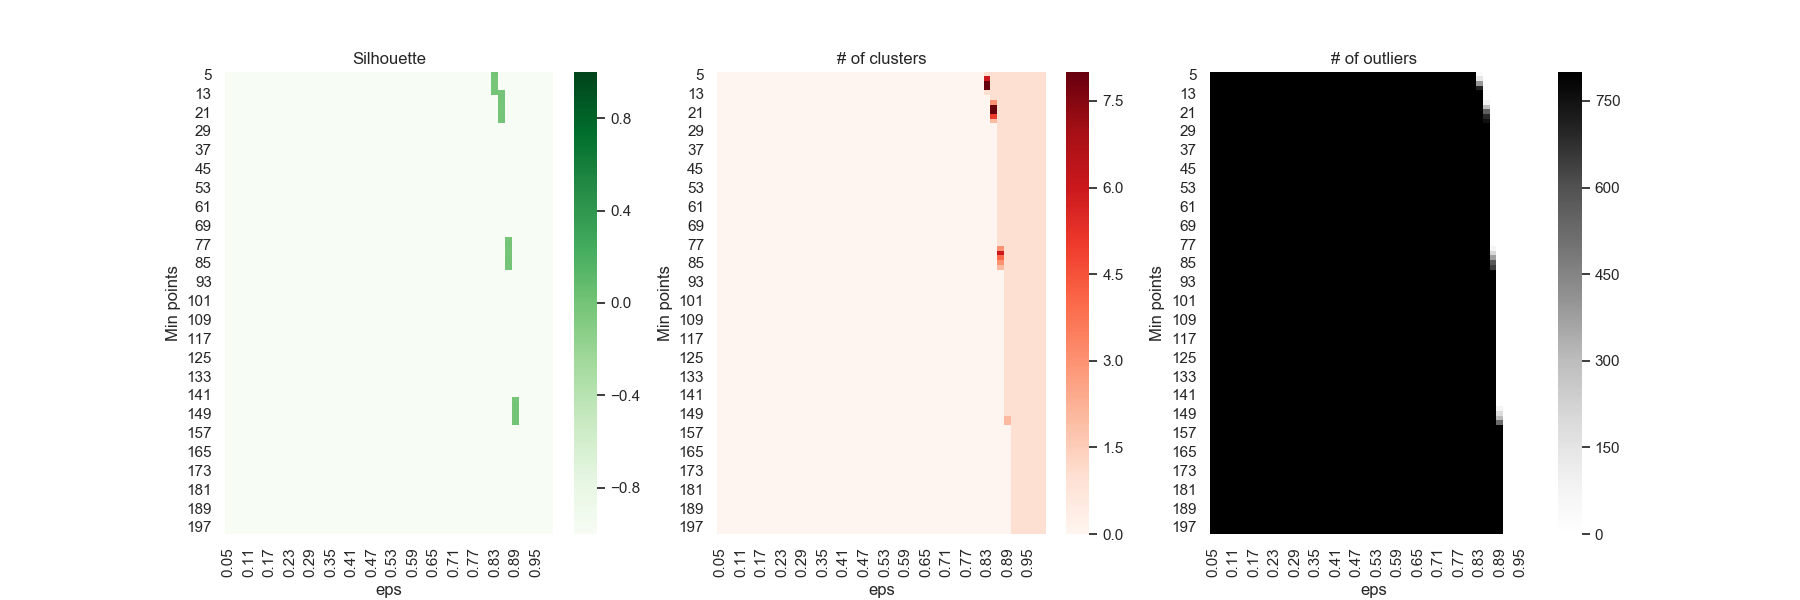
\includegraphics[width=\textwidth]{figures/RandHigh.png}
         \caption{Random (high) validator selection}
         \label{fig:DBRANH}
     \end{subfigure}
        \caption{The silhouette, number of clusters and number of outliers for different values of $eps$ and $minPts$ for synthetic data.}
        \label{fig:dbRan}
\end{figure}

\section{Correlation matrix}
\label{sec:cm}
While the similarity between the round validator vectors can be assessed using the clustering based technique, the collusion factor can be guessed but not really visualised. This collusion factor is high when the presence of a given subset of the validators constantly co-occurs with the presence of another well defined subset. In other word when, in the round, there is a correlation between the presence of one validator and another. In order to depict this, we propose to build and visualise the correlation matrix (Pearson correlation) between the validators based on the round vectors. Figures \ref{fig:CORRARK} and \ref{fig:CORRLISK} show the correlation matrices (left) of the validators computed using the day-based sampling. A bright yellow indicates highly positively correlated validator (i.e. usually present together) while light blue indicate a random correlation and dark blue indicates high negative correlation (i.e., always not present together). The matrices on the right depicts the p-values which reflects the significance of the correlations with values lower than 0.05 mean a high significance.
It is clear that, in the cases of both ARK and LISk, some validators are correlated one to the other. Although, the correlations in the LISk case are more pronounced whether at the launch of the blockchain due to the long usage of genesis validators\footnote{ARK also had a full list of genesis validators at the launch (top left corner), however, their presence in the system was for short in time, which render them more likely to be eliminated upon the sampling process.} or at the end where a new coalition seems to start emerging (bottom right corner).  A discussion on the important tempoal aspect is given further in this document.

\begin{figure}
     \centering
     \begin{subfigure}[b]{\textwidth}
         \centering
         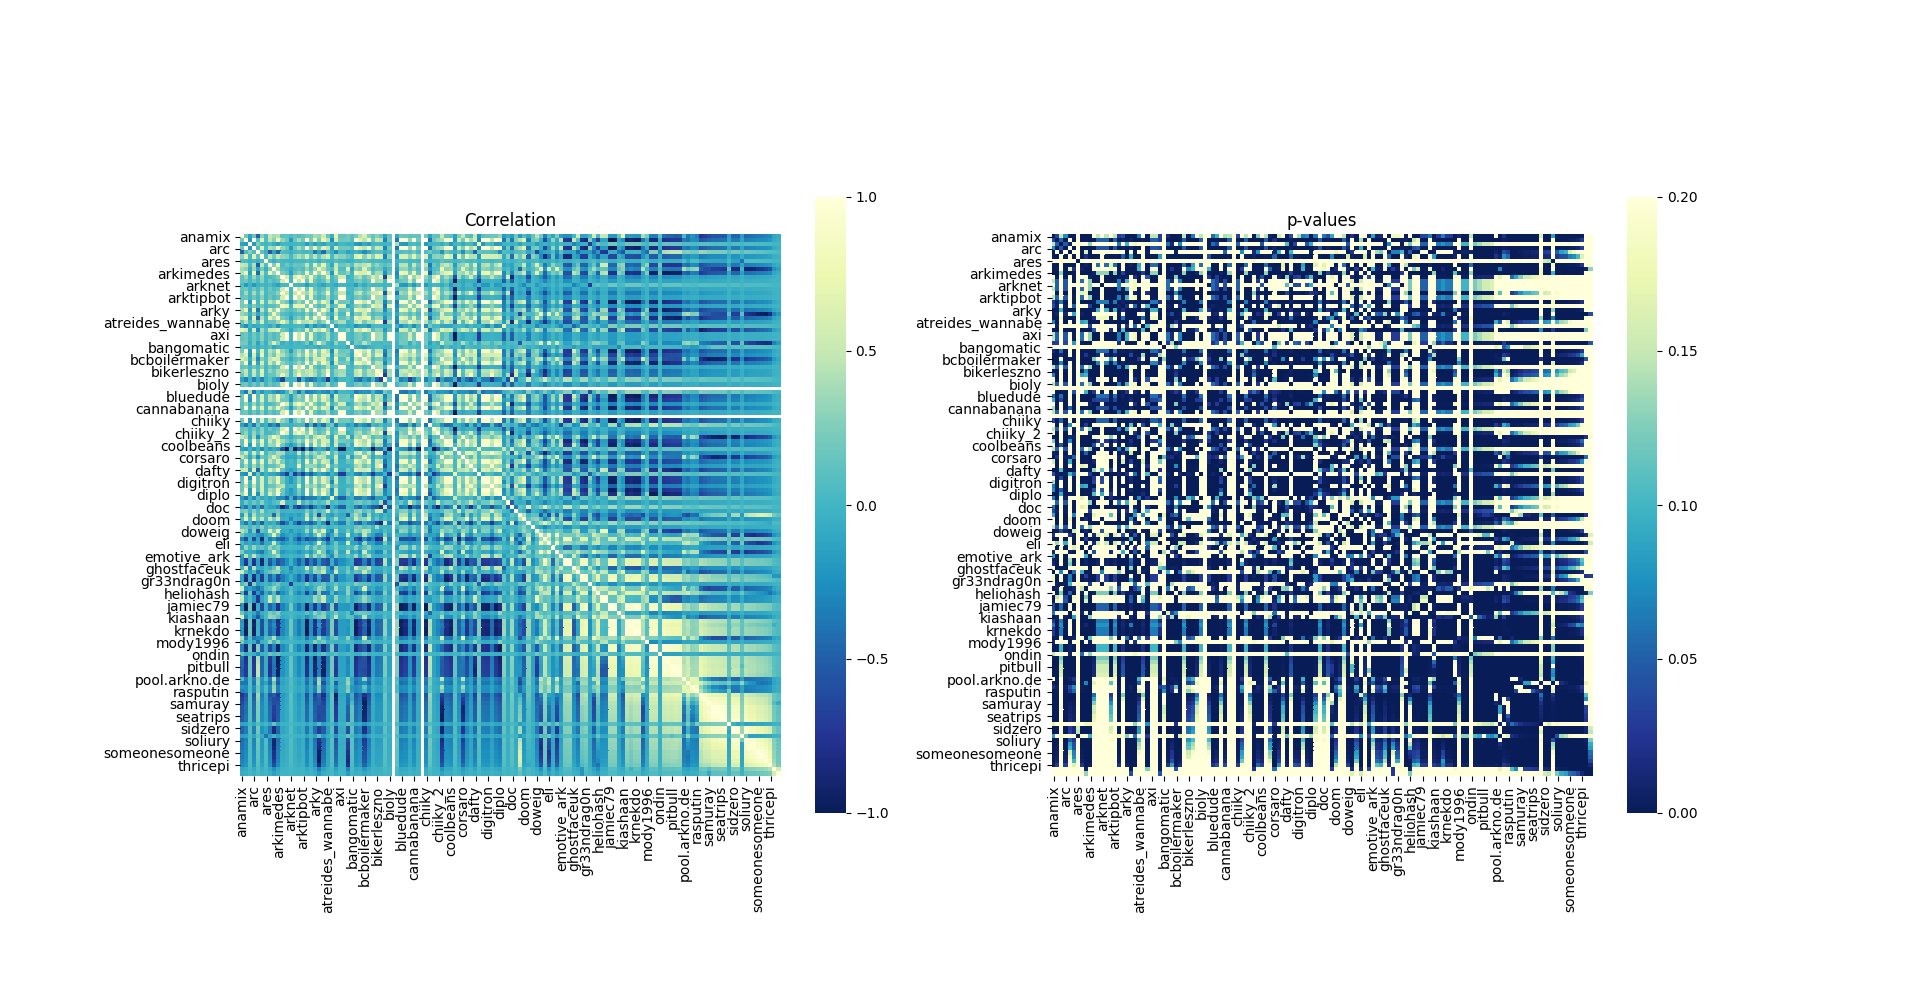
\includegraphics[width=\textwidth]{figures/ARKWeekReal.png}
         \caption{Validator selection in ARK}
         \label{fig:CORRARK}
     \end{subfigure}
     \hfill
     \begin{subfigure}[b]{\textwidth}
         \centering
         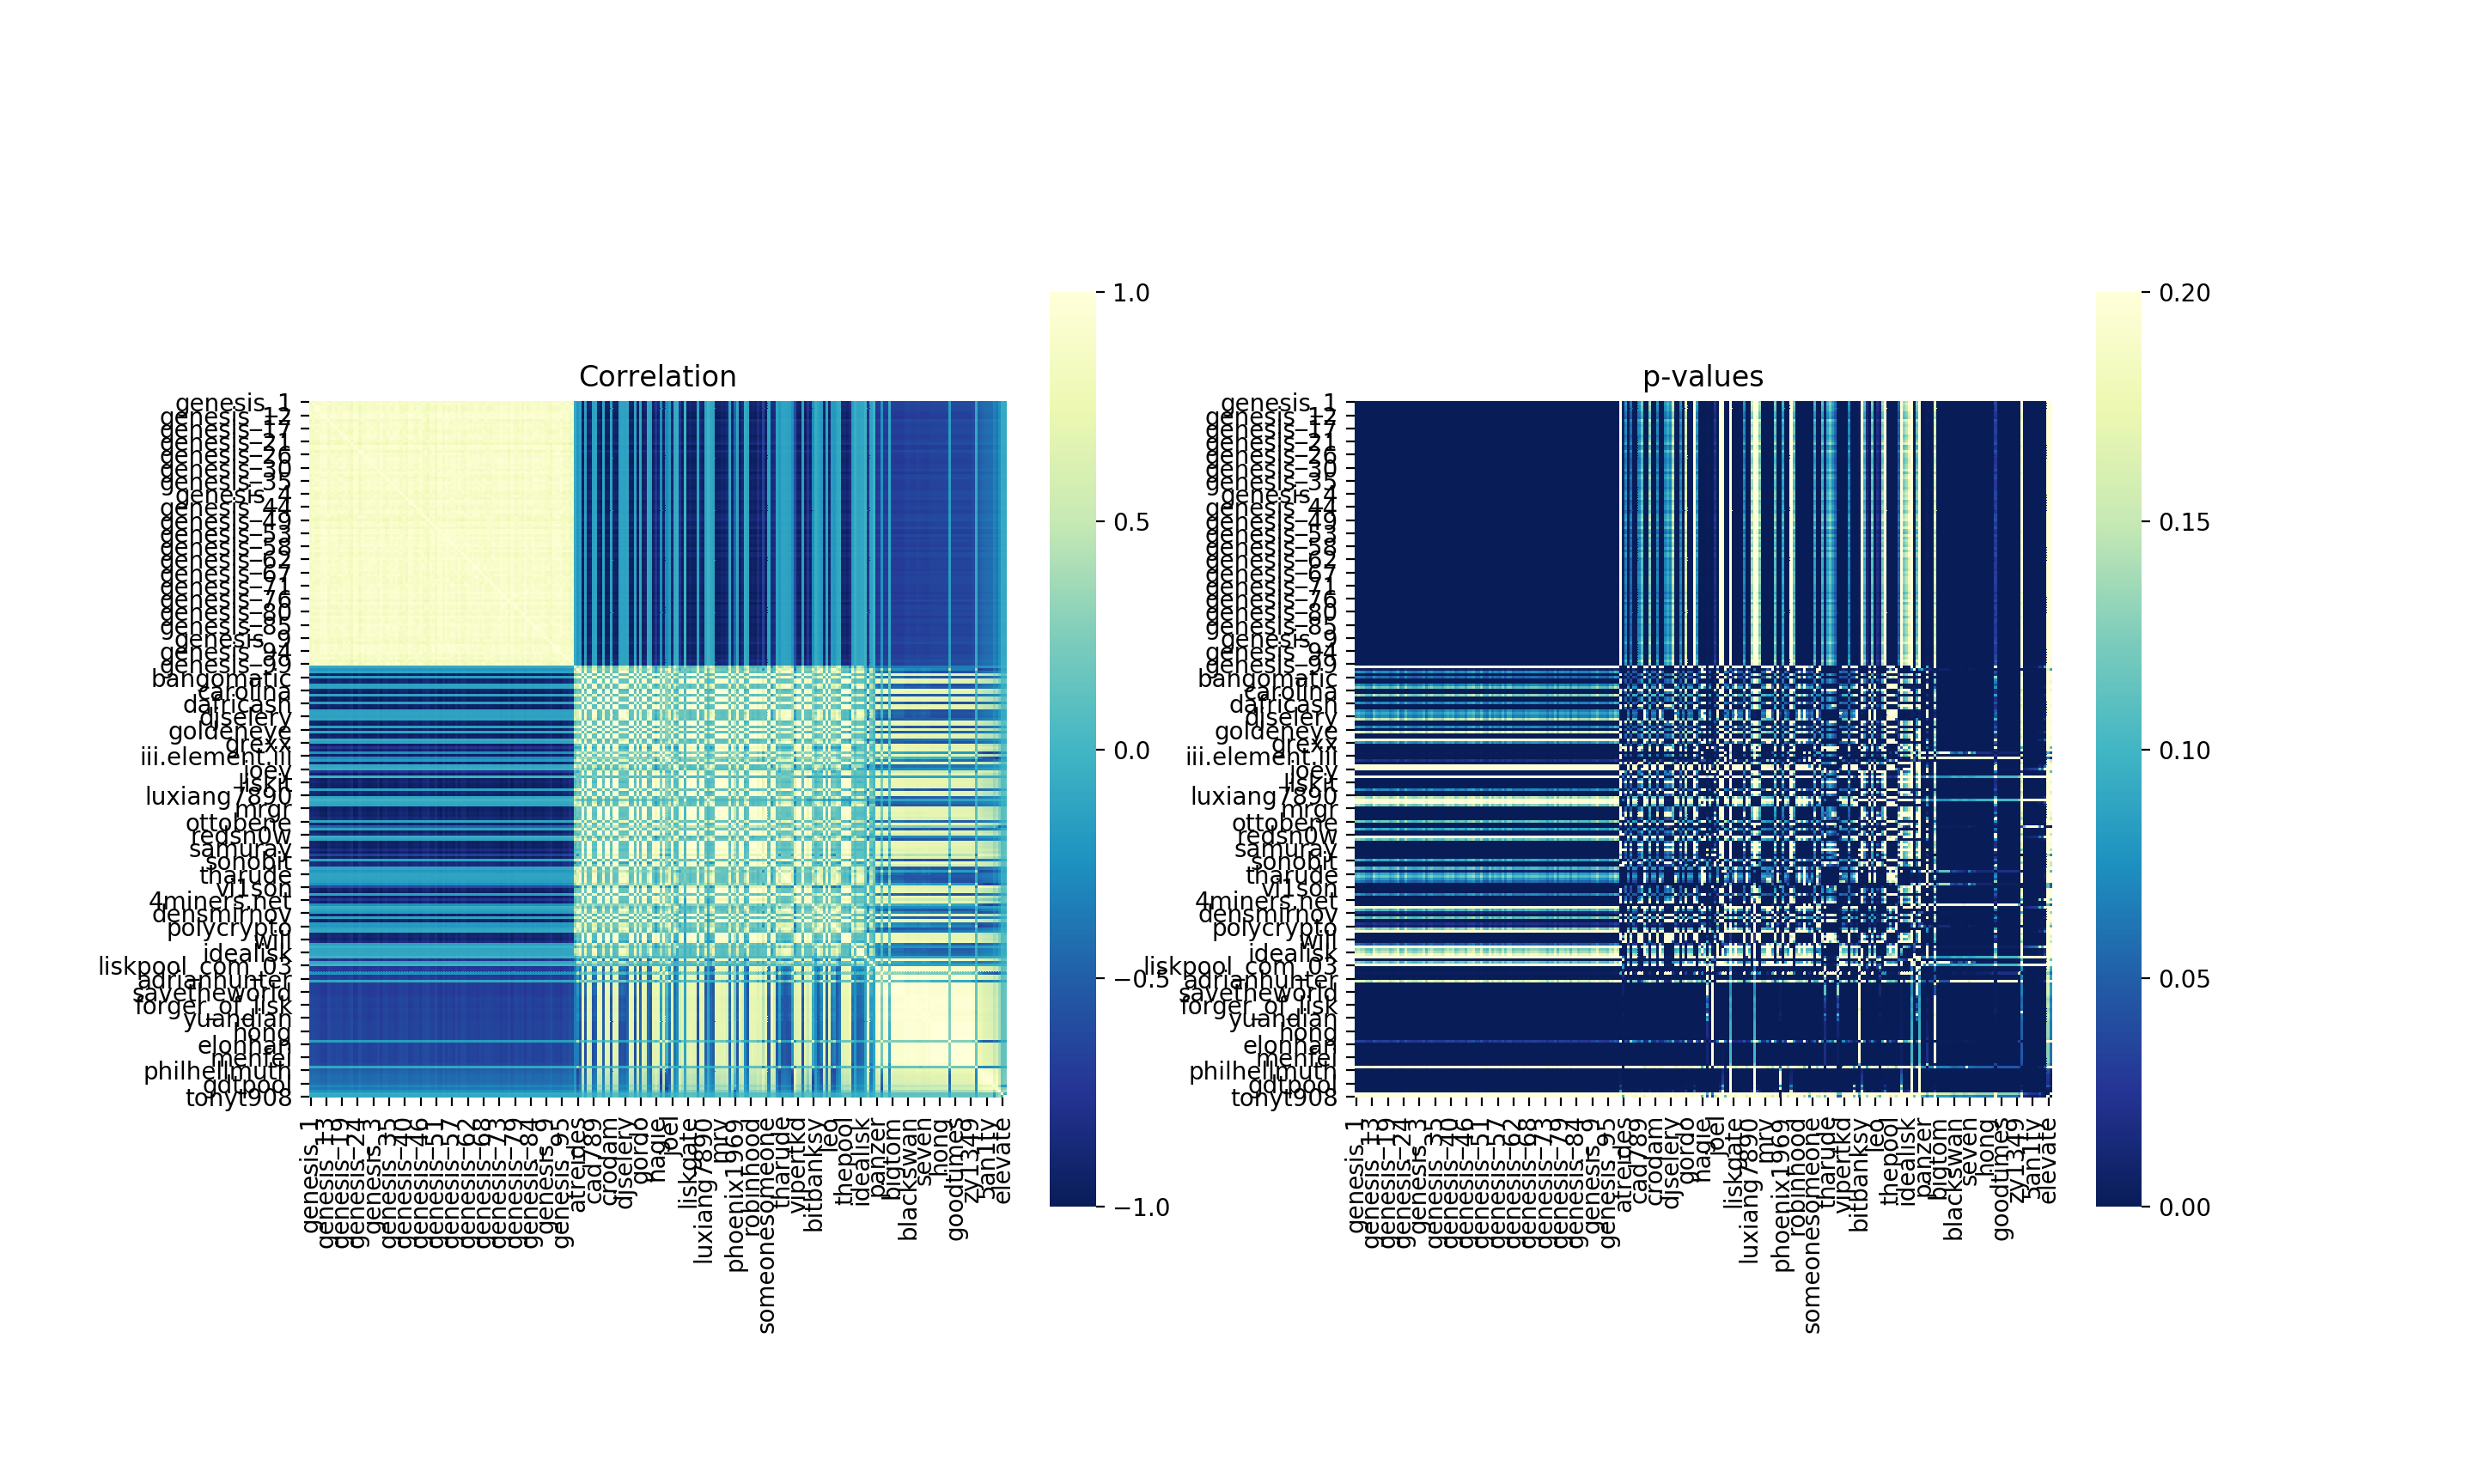
\includegraphics[width=\textwidth]{figures/LISKWeekReal.png}
         \caption{Validator selection in Lisk}
         \label{fig:CORRLISK}
     \end{subfigure}
        \caption{The correlation matrix (left) and the p-value matrix (right) of the round validators.}
        \label{fig:three graphs}
\end{figure}


\section{Limitations}
The approaches described in this document strive to empirically show the decentralization degree of a given DPoS based blockchain. While they allow to capture the concentration of the validation power, some of these approaches, either ignore the temporal aspect - which is a key element in measuring the decentralization - or deal with it in a basic manner.

\paragraph{Krippendorff's alpha} It is clear that the input of the alpha measure computation does not explicitly provide the temporal information. Indeed, when a round $n$ and a round $n + k$ disagree (or agree) to the same extent on the validators they include, this will impact the final value of alpha in the same manner regardless the value of $k$. In other words, one cannot capture the presence of changes close in time (between 2 rounds) and changes far in time (between year 1 and year 2 for instance). However, one can argue that the final - highly compact - representation of the centralization degree (i.e. the alpha metric) can be easily adapted to account for this temporal information by computing it for different epochs of the blockchain lifetime. This would lay a vector whose values should be closer to 0 to indicate a trully decentralized system\footnote{One can also compute the distance between the vector and the Zero vector}.

\paragraph{Clustering based approach} The round vectors considered as input to the density based clustering lack for the temporal dimension. Thus, the output of the clustering process only reflects the concentration of the validation power but does not reflect its changes in time. Hence, conclusions regarding the security risks and the accountability (e.g. how the voting process drives the validators in and out of the system) cannot be made. One way of remedying to this is to cluster the rounds not only w.r.t. their similarity but also w.r.t. their occurrence time through a two-stage clustering process.

\paragraph{Correlation matrix} In contrast with the first two approaches, the correlation matrix captures one element of the temporal dimension. That is the relative arrival time of a given validator w.r.t. the other validators. This shows the global drift of the concentration of the validation power from one group (e.g. genesis validators) to another group. This, in turn, reflects the existence of "validation epochs" (i.e., long periods of time during which the validators stay relatively unchanged between rounds.). The number of these epochs (which can be used as an input to the epoch-based alpha computation explained earlier) shows the balance between the stability of the system and its decentralization.

The round vectors considered all through this document constitute in reality a time series. Therefore, one can leverage the myriad of existing time series mining techniques to identify interesting sub-sequences and concept drifts that allow to better identify the risk factor (e.g. the stationary votes and the whale dominance) in a given blockchain.
\section{Conclusion}
\label{sec:conclusion}
In this document, we proposed a set of descriptive methods to measure and compare the decentralization of DPoS based systems. The experiments showed that these measures are capable of capturing centralization pattern in common DPoS blockchains such as high stability duration and high concentration of validation power. This can be later mapped to security concerns and thus helps conceive more resilient and secure DPoS systems.

We are working on more extensive evaluations of these measures which, despite being basic, seem to be capturing enough information about the decentralization in the studied blockchains. Indeed, other situations (e.g., subset collusion, partial randomness, ...) need to be studied to prove that the measures and techniques are able to capture them. The aim of this work is to prepare the ground for building the evaluation block of Ki's Proof of reputation consensus (PoR) simulator which in turns will be used to test and tune our PoR algorithm and its parameters.

\bibliographystyle{plain}
\bibliography{references}
\end{document}
